\chapter{Data Collection and Analysis}
\label{ch:DataAnalysis}
\thispagestyle{empty}


%%%%%%%%%%%%%%%%%%%%%%%%%%%%%%%%%%%%%%%%%%%%%%%%%%%%
%%%%%%%%%%%%%%%%%%%%%%%%%%%%%%%%%%%%%%%%%%%%%%%%%%%%
%%%%%%%%%%%%%%%%%%%%%%%%%%%%%%%%%%%%%%%%%%%%%%%%%%%%

\section{Thermal Analysis Methods}
\label{chap:TA-methods}

%%%%%%%%%%%%%%%%%%%%%%%%%%%%%%%%%%%%%%%%%%%%%%%%%%%%
%%%%%%%%%%%%%%%%%%%%%%%%%%%%%%%%%%%%%%%%%%%%%%%%%%%%
%%%%%%%%%%%%%%%%%%%%%%%%%%%%%%%%%%%%%%%%%%%%%%%%%%%%

\section{VASE and Modeling}

Ellipsometry was used extensively to determine a variety of properties of the material. However, the primary goal of ellipsometric analysis was to determine the film thickness, in order to be able to determine the film growth rate (in terms of \AA\ per deposition cycle) of the process. 

%%%%%%%%%%%%%%%%

\subsection{Data Collection}

In order to collect the experimental data, the following series of steps were followed:

\begin{enumerate}
	%
	\item
	Optics alignment
	\item
	Ambient light compensation (DC offset)
	\item
	Data collection at multiple angles
	%
\end{enumerate}

Alignment of the optics of the system is performed in the manner described in the ellipsometer manual.\cite{WVASE-manual} The system can have focusing optics installed which diminish the spot size of the analysis, which is useful if inhomogeneity is expected in the sample as this is a major problem for analysis (two of the main assumptions made by ellipsometric models are that the layers have consistent thicknesses and optical behavior across the analysis area). This is done by manually adjusting the sample stage height and the sample surface plane. The system is designed so that when the incoming signal is maximized the sample is properly aligned with respect to the p- and s-planes defined by the equipment. 

Once the system is aligned, the signal that is due to ambient light (not produced by the light source) must be compensated for. The M-2000U defines this as the ``DC offset.''\cite{WVASE-manual} The offset is calibrated automatically by the system by blocking the light source and measuring the signal from the surroundings. As the light present in the room is generally randomly polarized, the signal will be invariant to the polarizer settings. Correctly setting this value greatly decreases the uncertainty during the analysis phase; it mainly affects the degree of light depolarization measured by the system. The ellipsometer includes the depolarization in its calculation of the confidence interval for the final measurement. If the degree of ambient unpolarized light is not determined before the measurement, the depolarization will be nearly completely unrelated to the actual depolarization by the sample. In addition, the depolarization can be used by non-idealized models to determine such parameters as layer thickness variation, or internal interface roughness. This process will not be used for the remainder of this discussion, but more information can be found in the manual for the M-2000U.\cite{WVASE-manual} 

After the calibration steps have been completed, data collection can be performed. Three different incident angles were used for the data collection: 55\Deg{}, 60\Deg{}, and 65\Deg{}. At each angle, the data was averaged over three hundred revolutions of the compensator to minimize noise in the experimental data. The system was set up to collect depolarization data simultaneously with the ellipsometric parameters.\cite{WVASE-manual} 

If the sample is expected to be inhomogeneous, the focusing optics can be used and data collected at several different locations on the sample. This can provide data on how the growth process behaves spatially, such as if there is abnormal growth near the edges of the sample but homogeneous deposition as one moves nearer to the center of the substrate. 

%%%%%%%%%%%%%%%%

\subsection{Model Definition}

The definition of the model is a critical part of the analysis procedure. The model dictates how the software package will perform its various calculations to predict the overall optical behavior, which it iteratively compares to the experimentally determined $\psi$ and $\Delta$. 

Simply put, the model is defined as a bulk (semi-infinite) substrate layer, with a nominal number of nano- to micrometer thick layers stacked upon it. Each layer is modeled with a prediction of optical constants at each test wavelength. These optical constants can be provided as a table of experimentally determined results, which are available for many commonly used materials such as silicon, silica, titania, amongst others; they can also be predicted using a variety of different models. These can be empirical predictors, such as the Cauchy dispersion, or based upon physical properties of the material, oscillator-based models for example. The model types relevant to this work are discussed in more detail in subsequent sections. 

The four different substrates require different material layer stacks to properly represent them, and each poses individual challenges for characterization. The Si(100) substrate that was most commonly used for this work was the simplest to model. It can be represented as a substrate layer of silicon, with a 200nm layer of silica on top. The deposited film would be layered above the \ce{SiO2} layer (see fig.~\ref{fig:Si(100)-model} for a schematic representation). A large number of these substrates were analyzed for their oxide layer thickness, where the only parameter to be fit was the layer thickness. It was found that the nominal oxide layer was 200 $\pm$ 5nm thick. This was consistent enough that 200nm could be used for the initial thickness estimate for all samples using this substrate, and after the ALD layer was analyzed this thickness could also be included in the fit to confirm the true dimensions of the oxide layer. The substrate with thermally-grown oxide was preferred in comparison to silicon with only native oxide layer; this is because the thicker layer of transparent oxide helps to generate large oscillations in $\psi$ and $\Delta$, which assists in the analysis (particularly the thickness, where the fringes are very closely related to this parameter). 

\begin{figure}[htbp]
   \centering
   \includegraphics[width=0.5\textwidth]{./figures/DataAnalysis/ellipsometry-model}
   \caption[Graphical Schematic of VASE Model]{A simple graphical example of the model used for %
   					analysis of the film stack in the Si(100) samples. The unknown parameters %
					are $t$ and the spectroscopic values of $\tilde{n}$ for the PTO layer.}
   \label{fig:Si(100)-model}
\end{figure}

%%%%%%%%%%%%%%%%

\subsection{Analysis Procedure}

Once the data was collected, a specific series of steps was followed in order to create the highest degree of accuracy from the model. All steps were performed on the PTO layer. The procedure went as follows:

\begin{enumerate}
\item
High-$\lambda$ Cauchy Model
\item
Direct Calculation of $n$ and $\kappa$
\item
Conversion to Oscillator Model
\item
Refinement of Oscillator Layer Parameters
\end{enumerate}

This first step takes advantage of the transparency of the film at high wavelengths (low energies) where the photon energy is below the optical bandgap of the material. In this region, the Cauchy model can be used. The Cauchy model is empirical rather than physically descriptive, and best used for amorphous materials such as polymeric films, however the assumptions required for reasonable accuracy are met when absorption in the film layer is minimized (therefore $\kappa(\lambda)\approx0$). The equations used in the Cauchy model are shown in equation~\ref{eq:cauchy}. Generally, analysis during this step was performed in the spectral region where $\lambda = 600-1000$nm ($E_{ph} = 2.06-1.24$eV). 

\begin{subequations}
\label{eq:cauchy}
\begin{align}
	n\left(\lambda\right) &= A_{n} + \frac{B_{n}}{\lambda^{2}}+\frac{C_{n}}{\lambda^{4}}+\cdots\\
        	\kappa\left(\lambda\right) &= A_{\kappa}e^{B_{\kappa}\left(\frac{hc}{\lambda}\right)-C_{\kappa}}
\end{align}
\end{subequations}

Once reasonable estimates for $n$, $\kappa$, and the film layer thickness are obtained at the higher wavelengths, the second step of the analysis is to generate values of $\tilde{n}$ for the rest of the spectrum. The film thickness parameter is fixed at the value determined from the Cauchy model. The values of $n$ and $\kappa$ are allowed to be determined freely without the use of a model (i.e. directly determined by use of the Fresnel relations). This type of modeling is not physical, but assists in the generation of the oscillator-based model in the next step. The software package is then instructed to run a point-by-point fit of the data from highest- to lowest-$\lambda$, attempting to minimize the change in $n$ or $\kappa$ between adjacent data points. 

This model is then inputted into a oscillator model. For the analysis of these films, a Tauc-Lorentz oscillator model was utilized. The oscillator models used by WVASE32 are expressed in terms of the complex dielectric function $\tilde{\epsilon}$, which relates to $\tilde{n}$ via the relationship in equation~\ref{eq:dielectric}. The Tauc-Lorentz model changes the Lorentzian model by allowing for some absorption below the fundamental bandgap energy, which would be due to defect states and other intra-band transition mechanisms. The Tauc-Lorentz model uses the parameterization shown in equation~\ref{eq:TaucLorentz}\cite{WVASE-manual,Jellison96}. $\epsilon_{1}$ is provided here in a condensed version (eq.~\ref{eq:TaucLorentz-1}); the full expanded version, and its derivation via Kramers-Kronig integration from $\epsilon_{2}$, has been presented by Jellison and Modine\cite{Jellison96}. 

\begin{subequations}
\label{eq:dielectric}
\begin{align}
	\tilde{\epsilon} &= \epsilon_{1}+i\epsilon_{2} = \tilde{n}^{2}\\
	\epsilon_{1} &= n^{2} - \kappa^{2}\\
	\epsilon_{2} &= 2n\kappa 
\end{align}
\end{subequations}

\begin{subequations}
\label{eq:TaucLorentz}
\begin{align}
	\label{eq:TaucLorentz-1}
	\epsilon_{1}=\frac{2}{\pi}P\int^{\infty}_{E_{g}}\frac{\xi\epsilon_{2}\left(\xi\right)}{\xi^{2}-E^{2}}\,%
				\mathrm{d}\xi & \hspace{2.5cm}
\end{align}
\begin{empheq}[left=\empheqlbrace]{align}
	\epsilon_{2} (E) = \frac{AE_{0}C\left(E-E_{g}\right)^{2}}{\left(E^{2}-E^{2}_{0}\right)^{2}+C^{2}E^{2}}%
		\cdot \frac{1}{E} && E> E_{g}\\
        	\epsilon_{2} (E) = 0 && E\leq E_{g}
\end{empheq}
\end{subequations}
\\
\indent The WVASE32 software package allows one to use a graphical interface to provide initial guesses for the various fit parameters. At times this required multiple oscillators to best fit the predicted $\epsilon_{2}$ function. Once this has been set, all of the parameters affecting $\epsilon_{2}$ ($A, E_{0}, C, E_{G}$) are marked to be included in the fit. The software is then instructed to perform a best-fit of the oscillator to $\epsilon_{2}$. Once this operation completes, the software is set to fit to $\epsilon_{1}$ and only the value of the $\epsilon_{1}$ offset is allowed to be fit. Finally, the software is set to optimize vs both $\epsilon_{1}$ and $\epsilon_{2}$, and all parameters are included. This completes the initial setup of the oscillator model. 

Finally, the model is set to also allow the layer thickness to be fit and a general fit to the entire experimental dataset is performed. This provides the best guess to the physical values of the film. The thickness calculated by this procedure matches very closely to measurements performed by other methods (e.g. SEM imaging or AFM measurement of a lithographically created step). The bandgap parameter also matches well to literature values (when using standard samples of well defined materials, such as a thin layer of titania). 

If similar deposition parameters are utilized, it is possible to save the parameterized model for later use. This allows the analysis to be streamlined when the material is expected to remain constant, for example if tests of deposition at different layer thicknesses are performed. In this case, the material would have optical behavior very similar to the initial sample, and the oscillator model would be sufficiently close to valid parameters to be used directly for fits. All that would need to be adjusted initially would be the estimated layer thickness. If the fit fails to produce useful data, such as unreasonable values for any of the parameters or very large confidence intervals, it is recommended to proceed with the entire standard analysis procedure. 

Experimental data sets and the resulting fitted model for selected samples are presented in appendix~\ref{sup:Ellipsometry}.

%%%%%%%%%%%%%%%%%%%%%%%%%%%%%%%%%%%%%%%%%%%%%%%%%%%%
%%%%%%%%%%%%%%%%%%%%%%%%%%%%%%%%%%%%%%%%%%%%%%%%%%%%
%%%%%%%%%%%%%%%%%%%%%%%%%%%%%%%%%%%%%%%%%%%%%%%%%%%%

\section{Composition Analysis}

In order for the desired phase to be preferred, without any impurity phases precipitating, it is important to be able to control the stoichiometry of the produced film. Previous reports have shown that there is a close relationship between the composition of the film and the final resultant phase (see figure~\ref{fig:PTO-phase}). 

\begin{figure}[htbp]
   \centering
   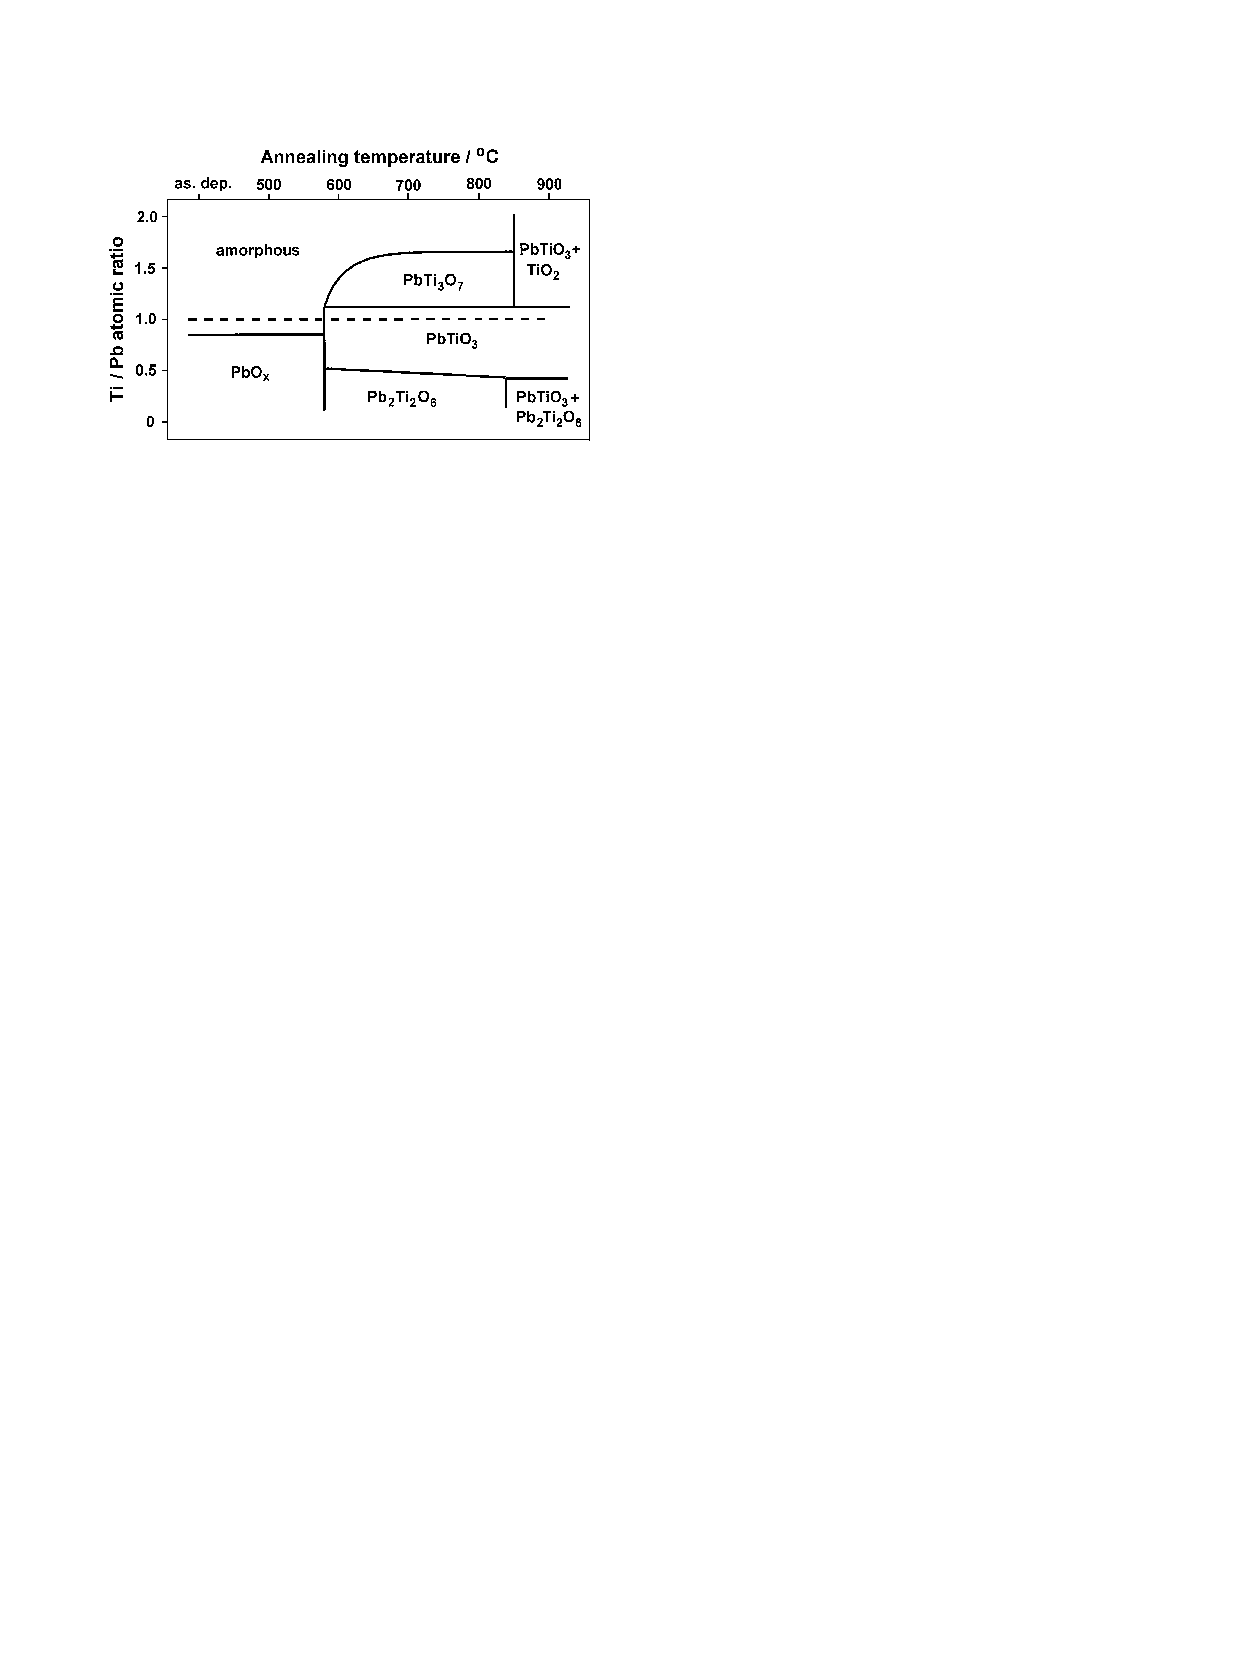
\includegraphics[width=0.75\textwidth]{./figures/dataanalysis/PTO-phase}
   \caption[Preferred Phase vs. Stoichiometric Ratio]{Graphic illustrating preferred phase of an annealed %
   		film at a range of stoichiometric ratios and annealing temperatures. A slight excess of \ce{Pb} %
		in the system helps to stabilize the perovskite \PTO{} phase.\cite{harjuoja_2006}}
   \label{fig:PTO-phase}
\end{figure}

\lipsum

%%%%%%%%%%%%%%%%

\subsection{Energy-Dispersive X-Ray Spectroscopy}



\lipsum

%%%%%%%%%%%%%%%%

\subsection{X-Ray Fluorescence Spectroscopy}

\lipsum

%%%%%%%%%%%%%%%%%%%%%%%%%%%%%%%%%%%%%%%%%%%%%%%%%%%%
%%%%%%%%%%%%%%%%%%%%%%%%%%%%%%%%%%%%%%%%%%%%%%%%%%%%
%%%%%%%%%%%%%%%%%%%%%%%%%%%%%%%%%%%%%%%%%%%%%%%%%%%%

\section{X-Ray Diffraction}

\lipsum

%%%%%%%%%%%%%%%%

\subsection{Grazing Incidence XRD}

\lipsum






